\documentclass[11pt]{scrartcl}
\usepackage{answers}
\Newassociation{sketch}{hintitem}{hints}
\renewcommand{\solutionextension}{out}

\usepackage[sexy]{evan}
\newcommand\EE{\mathbb E}
\newcommand\PP{\mathbb P}
\usepackage{graphicx}
\usepackage{wrapfig}
\begin{document}
\title{Image Depth Estimation Using Stereo Vision}
\author{Mrinall Umasudhan}
\date{April 25, 2022}
\maketitle
\Opensolutionfile{hints}

\begin{abstract}
  Candidate ID: \mailto{943289432}.
\end{abstract}

%TOC
\tableofcontents

% EV.pdf
% ploh handouts

\newpage

\section{Introduction}
One of the most explored problems in the field of computer vision is the process
of accurately estimating the real-world depth of a pixel within a two dimensional
image. The inference of three dimensional information is done by using multiple two
dimensional views of a scene, the process being deemed the name stereo vision.

\subsection{Applications}
A common counter-argument to the practicality of stereo vision algorithms
are the presence of other sensors that do not make use of visual data such
as ultrasonic or time of flight distance sensors. While these sensors are not
not impacted by factors that would be detrimental to the accuracy of stereo
vision algorithms such as the lack of adequate lighting,
"stereo vision has the advantage that it achieves the 3-D acquisition without
energy emission or moving parts" (https://research.csiro.au/qi/stereo-vision/). Moreover,
whereas traditional distance sensors focus on a singular point in space, stereo vision
algorithms are only limited by the camera's field of view, making the depth analysis
large area far more simple and cost effective. Finally, stereo vision algorithms are able
to easily work in conjunction with other
computer vision techniques such as machine learning based object detection
models when compared to the previous depth estimation approaches as it already
tracks depth on the same image plane that a object detection model may be implemented on.
These factors allow for a far greater analysis of the
various shapes and angles in an image leading to its usage in various fields.
\\
\begin{wrapfigure}{R}{0.5\textwidth}
  \centering
  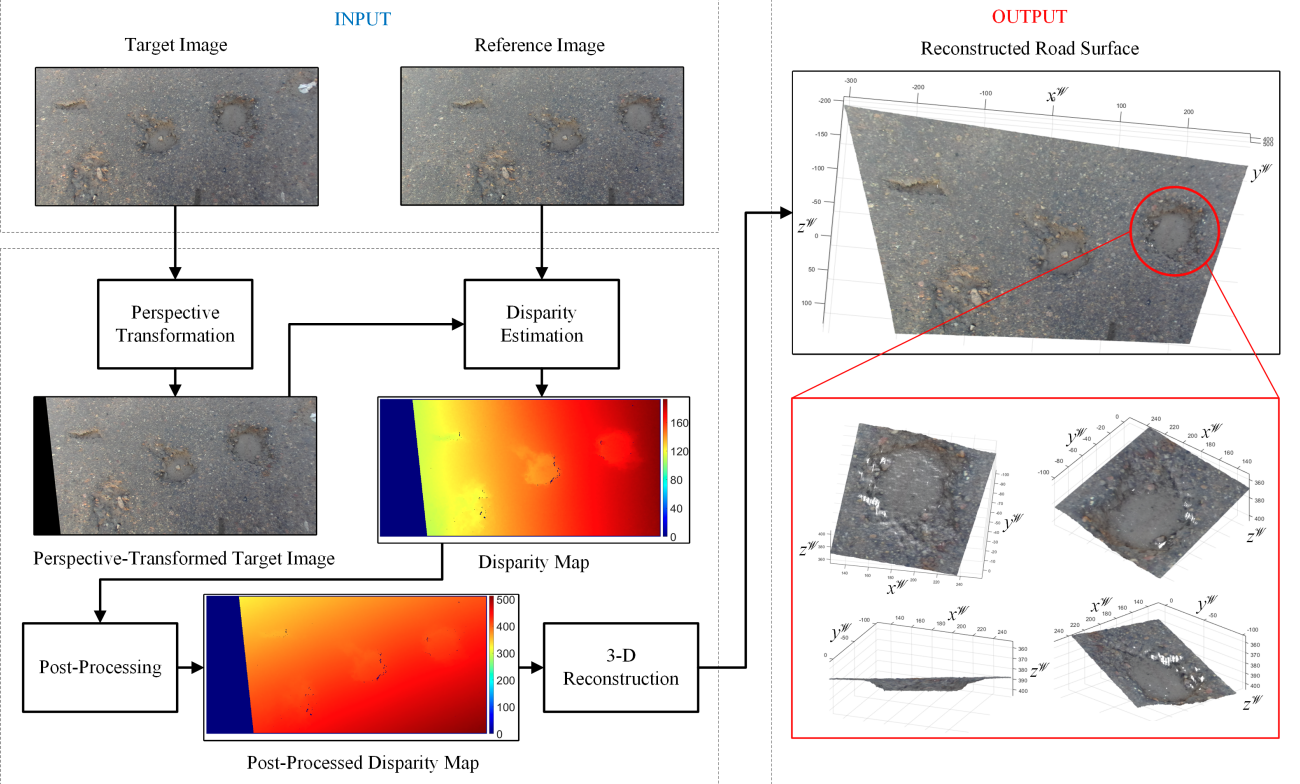
\includegraphics[width=0.5\textwidth]{img1.png}
  \caption{\label{fig:frog1}Stereo Vision For Road Deformity Detection}
\end{wrapfigure}

A common application of stereo vision algorithms is in the quality
control process of industrial factories. Factories must analyze each
finished product for deformities in order to maintain a standard of quality in their
products. However, many factories output a high volume of product every day meaning that
the human analysis of such product would be far too expensive and inefficient when
considering the large amounts of workers needed to manually inspect each products
as well as the time it takes for the inspection of a product. The installation of multiple
distance sensors in order to analyze each square inch of a product would also be far too expensive.
However, because a factory is in a controlled environment with uniform lighting and the object is one
of known shape, the usage of a stereo vision algorithm would be ideal for the situation as stereo cameras
are able to analyze objects with their large field of view and can easily detect deformities as the object
being analyzed is of known geometry, meaning the algorithm can compare each depth point of the current object
to the depth of a model product, reporting any deformities both accurately and efficiently.  and can easily detect deformities as the object
being analyzed is of known geometry, meaning the algorithm can compare each depth point of the current object
to the depth of a model product, reporting any deformities both accurately and efficiently. \\

A paper done by the University of Bristol explored deformity analysis preformed by stereo algorithms
further by acquiring three dimensional road data for autonomous cars further displaying the
capabilities of stereo algorithms. The process which this algorithm follows can be seen in the
figure above.

\subsection{Overview and Purpose}

The essence of many successful stereo vision algorithms can be summarized in three key steps:

 
  \paragraph{ Triangulation} The process of assigning depth values to each pixel in the image
        using multiple two dimensional views of a scene and the specific parameters from
        camera hardware, difference in location of the cameras used, and the disparity in the
        pixels from each view of the scene.
    \paragraph{ Calibration} The process of correcting image distortion caused by the
        spherical geometry of the camera lens
        and reifying the two dimensional views of the scene such that
        the objects in study are on the same plane.
  \paragraph{Pixel Correspondence} In order to apply the triangulation process the algorithm must be
        able to match a pixel from one view of the scene to another view taken from a separate camera
        also known as the disparity value of this pixel.
\\

\\

In modern research, the most studied step of the algorithm is the process of pixel Correspondence,
better known as stereo matching. As of now there are many optimization techniques being applied
to stereo matching algorithms in order to increase their efficiency and accuracy. Firstly, this paper explains
the math and logic behind each portion of a successful stereo vision system while providing implementations.  finding value in optimization techniques
when compared to more standard stereo matching approaches. In order to analyze and implement a sound stereo vision algorithm
as well as a optimized matching algorithm scholarly sources were regarding stereo vision and optimization
techniques for pixel correspondence. After implementing a standard matching algorithm as well as another using
the optimization technique known as dynamic programming, I found that there was a significant increase
in both accuracy and efficiency in the depth estimates provided from the algorithm.


\section{Triangulation}

The core of every stereo vision algorithm is to find the depth of a pixel
using multiple two dimensional views of the scene, more formally
this process is known as the backwards projection of a camera from image
coordinates into three dimensional world coordinates. In order to derive the
formulas for the backwards projection of a camera, the formulas by which
a camera uses in order to map world coordinates into image coordinates; this
process can be explained as the forwards projection model.
\subsection{Forward Projection Model}

Formally defined, the forward projection model "describes the mathematical relationship
between the coordinates of a point in three-dimensional space and its projection onto the image
plane of an ideal \textbf{pinhole camera}, where the camera aperture is described as a point and no lenses
are used to focus light" (\textbf{wikipedia}). The usage of a pinhole camera allows
for the elimination of lense distortion when mapping to the image plane, simplifying
the formulas significantly.

\begin{remark}
  The majority of cameras used in stereo vision algorithms, including those
  used in this paper, use lenses contradicting the pinhole camera model.
  However, because researchers calibrate their camera's in order to remove
  distortion from the images returned, the pinhole camera model can still
  be applied.
\end{remark}
The forward projection model of converting a 3D camera point into a 2D pixel
coordinate is defined using the formula below:
\begin{theorem}
  [Forward Projection Equation]

  \begin{displaymath}
    (u, v) = (f_x \cdot \displaystyle\frac{x_c}{z_c} + o_x,
    f_y \cdot \displaystyle\frac{y_c}{z_c} + o_y)
  \end{displaymath}
  \begin{figurekey}
    \begin{tabular}{llll}
      $(u,v)$ & two dimensional pixel coordinates        & $f_x$ & focal length on x-axis \\
      $x_c$   & $x$ position on scene coordinate frame   & $f_y$ & focal length on y-axis \\
      $y_c$   & $y$ position in scene coordinate frame   & $o_x$ & image center on x-axis \\
      $z_c$   & depth of point in scene coordinate frame & $o_y$ & image center on y-axis \\
    \end{tabular}
  \end{figurekey}
\end{theorem}
Whereas the other paramteres of the equation are self-explanatory, the focal
length ($f$) requires further explanation. The focal length is "the distance
between the lens and the image sensor when the subject is in focus" (Nikon Website).
As such, using this information the forward projection equations essentially show how
a ray from the camera to the scene is mapped to an image.


\subsection{Derivation of Backwards Projection Model}
It is clear that deriving the depth of a pixel from manipulating the forward
projection equations is impossible given the inquality in depth measurements
when using the $x$ and $y$ pixels. Therefore it is evident that additional
information is needed in order to infer depth. This is where the usage of
multiple viewpoints of a scene is needed.

\begin{remark}
  Although many stereo vision systems use more than two viewpoints of a scene,
  in order to simplify the implementation process a simple (binocular) stereo
  system will be used.
\end{remark}
\begin{wrapfigure}{R}{0.5\textwidth}
  \centering
  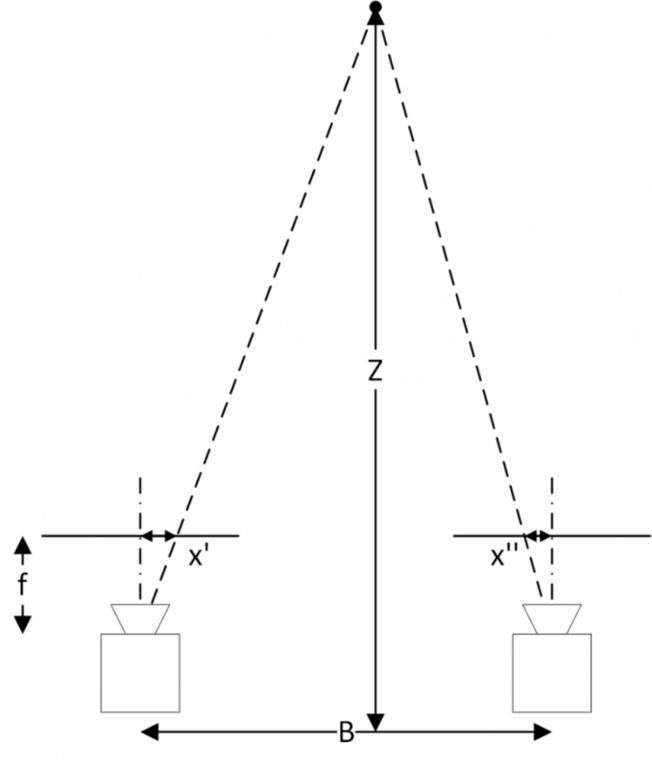
\includegraphics[width=0.3\textwidth]{img2.resized.png}
  \caption{\label{fig:frog2}Simple stereo system}
\end{wrapfigure}
\\
\\

As mentioned prior the forward projection equations essentially represent the camera
as projecting a ray from the image into a scene point. Using this fact, an
additional camera which is calibrated to be on the same plane as the original camera
may be used to project another ray from the corresponding image point onto the scene. By
finding the intersection of these two rays the depth of a pixel in the scene may be found. 
\\
Using the depth measurement of a pixel, it is also possible to derive
$(x, y)$ coordinates of a scene from the image coordinate frame, giving
the full scene coordinate frame:

\begin{theorem}
  [Backward Projection Equations]

  \begin{align}
    z & = \displaystyle\frac{b\cdot f_x}{(u_r-u_l)} \\
    x & = \displaystyle\frac{z}{f_x} \cdot (u_l - o_x) \\
    y & = \displaystyle\frac{z}{f_y} \cdot (v_l - o_y) 
  \end{align}

  \begin{figurekey}
    \begin{tabular}{llll}
      $(u_l,v_l)$ & pixel coordinates on left camera     & $f_x$ & focal length on x-axis \\
      $(u_r,v_r)$ & pixel coordinates on right camera   & $f_y$ & focal length on y-axis \\
      $x$     & $x$ position on scene coordinate frame  & $o_x$ & image center on x-axis \\
      $y$     & $y$ position in scene coordinate frame   & $o_y$ & image center on y-axis \\
        $z$     & depth of point in scene coordinate frame  &$b$ & baseline distance \\
    \end{tabular}
  \end{figurekey} \\ \\
    Note that the pixel coordinates in the left and right camera point at the same object in 
    the scene. However, because the cameras are located $b$ units away from each other, 
    the coordinates are unique creating the pixel coorespondance problem. 
\end{theorem}

The two rays projected from the camera, along with the calibrated basline measurement (distance
between left and right cameras) form a triangle, allowing for the derivations of the formulas
shown above. However, in order to attain the parameters in these formulas that are not 
immediatly present in the image such as focal length, and the baseline as well as correcting
for lense distortion camera calibration is required. Moreover, in order to make use of the ray 
projected from the additional viewpoint, the corresponding pixel from the right camera must be 
found with through additional algorithms. 


\section{Camera Calibration}

In order for the triangulation formulas to apply all cameras in the stereo 
system must be calibrated to match the pinhole camera model. This involves
finding the hardware parameters of the camera and correcting the images 
returned for lense distortion. Moreover, the images must be transfored such 
that they are displayed parallel to each other. 

\subsection{Intrinsic matrix}

A key step in correcting for lense distortion and applying the triangulation formulas
is identifiying the instrinsic parameters of both cameras. Formally explained, the 
instrinsic parameters are the variables used in the forward projection equations in order
to map 3D scene coordinates into image coordinates, such as the focal length and optical
center of the image. The intrinsic parameters of a camera are mathematically contained in 
a 3 by 3 matrix known as the instrinsic matrix. The forward projection equation can be 
rewritted in matrix form to show this: 

\begin{theorem}[Forward Projection Equation Matrix Variation]
     \begin{displaymath}
    \begin{bmatrix}
      u \\
      v \\
      w
    \end{bmatrix} &=
    \begin{bmatrix}
      f_x & 0 & o_x \\
      0 & f_y & o_y \\
      0 & 0 & 1
    \end{bmatrix}
    \begin{bmatrix}
      X \\
      Y \\
      Z
    \end{bmatrix} 
  \end{displaymath}
  \begin{figurekey}
    \begin{tabular}{llll}
      $(u,v)$ & two dimensional pixel coordinates        & $f_x$ & focal length on x-axis \\
      $X$   & $x$ position on scene coordinate frame   & $f_y$ & focal length on y-axis \\
      $Y$   & $y$ position in scene coordinate frame   & $o_x$ & image center on x-axis \\
      $Z$   & depth of point in scene coordinate frame & $o_y$ & image center on y-axis \\
    \end{tabular}
  \end{figurekey}

\end{theorem}

The parameters of the intrinsic matrix can be found by making use of the field of view 
and resolution of the camera of the camera, typically stated in the hardware specifications of the camera. The 
formulas are described below: 

\begin{theorem}
  [Instrinsic Matrix Calculation]

  \begin{align}
      f_x & = \displaystyle\frac{o_x}{\tan{\displaystyle\frac{a_x}{2}}} \\
    f_y & = \displaystyle\frac{o_y}{\tan{\displaystyle\frac{a_y}{2}}}  \\
    o_x & = \displaystyle\frac{r_x}{2} \\ 
    o_y & = \displaystyle\frac{r_y}{2} \\ 
  \end{align}

  \begin{figurekey}
    \begin{tabular}{llll}
      $(u_l,v_l)$ & pixel coordinates on left camera     & $f_x$ & focal length on x-axis \\
      $(u_r,v_r)$ & pixel coordinates on right camera   & $f_y$ & focal length on y-axis \\
      $x$     & $x$ position on scene coordinate frame  & $o_x$ & image center on x-axis \\
      $y$     & $y$ position in scene coordinate frame   & $o_y$ & image center on y-axis \\
        $z$     & depth of point in scene coordinate frame  &$b$ & baseline distance \\
    \end{tabular}
  \end{figurekey} \\ \\
    Note that the pixel coordinates in the left and right camera point at the same object in 
    the scene. However, because the cameras are located $b$ units away from each other, 
    the coordinates are unique creating the pixel coorespondance problem. 
\end{theorem}



\subsection{Extrinsic Parameters}

The extrinsic parameters of a camera refer to the position and orientation of the camera 
with respect to the world coordinate frame and corresponding cameras. In more complex 
stereo systems an extrinsic matrix is required, detailing the translation of the camera 
in the $x$, $y$, and $z$ axis as well as the roll, pitch, and yaw angles of the cameras. 
However, because a binocular stereo system is used, the two cameras are garunteed to 
be pointing in a straight line, while being on the same $y$ and $z$ axis leaving only 
a horizontal distance that can easily be manually computed. The baseline ($b$) is measured 
by finding the distance between the centers of the left and rightmost camera. 

\begin{remark}
    Becuase a simple stereo is used, the cameras are garunteed to be positioned 
    such the $y$ position of the camera is identical, removing the need of additional 
    calibration beyond the manual baseline measurement. 
\end{remark}

\subsection{Lens Distortion}
\begin{remark}
    Images from: https://www.tangramvision.com/blog/camera-modeling-exploring-distortion-and-distortion-models-part-i#tangential-de-centering-distortions
    \\ Text from: https://docs.opencv.org/4.x/dc/dbb/tutorial_py_calibration.html  
\end{remark}
The simple stereo model assumes that both cameras in use do not contain lenses. 
However, in real-world situations lenses must be present in order to ensure pixel 
quality. This results in two types of distortion which must be accounted for when
calibrating cameras.  
\paragraph{Radial Distortion}
    This variation of distortion causes "straight lines in images to appear curved" (h)
    Moreover, as pixels begin to deviate from the image center, distortion increases rapidly, 
    causing significant drops in accuracy when querying depth. 
\paragraph{Tangential Distortion}
    As opposed to radial distortion, tangential distortion causes some areas in the image to appear 
    closer than others due to the misalignment of the lense from the image plane. 
\\
\begin{figure}[!htb]
    \centering
    \subfloat[\centering Radial]{{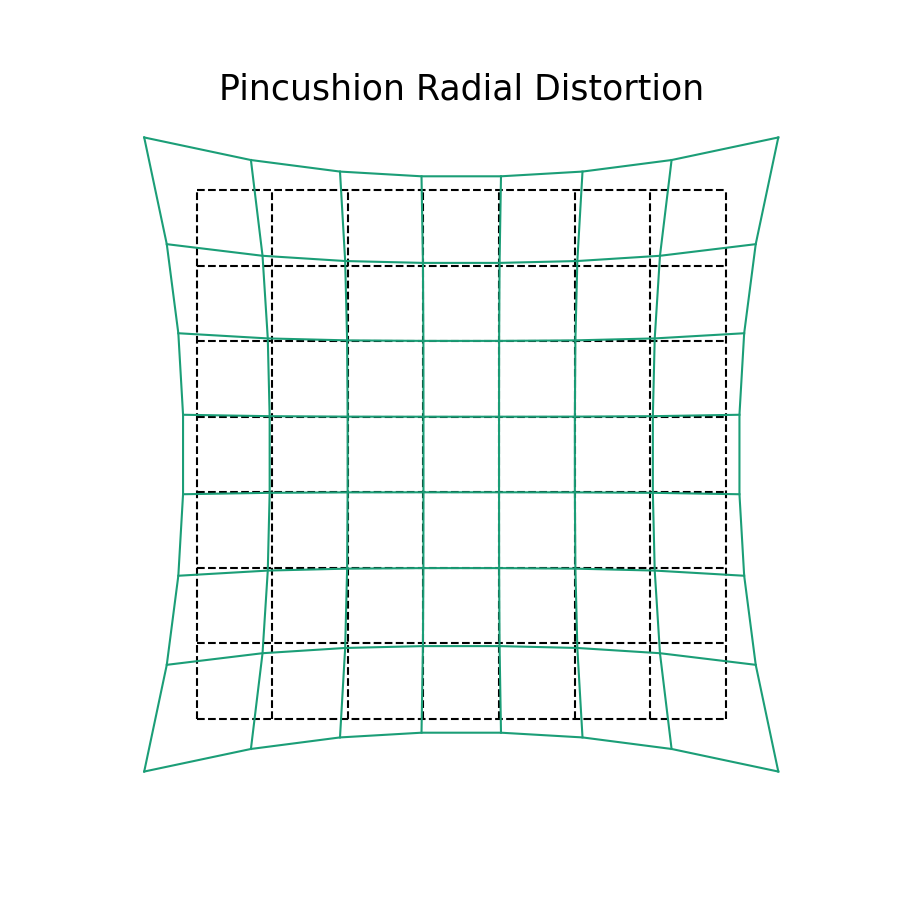
\includegraphics[width=4cm]{radial.png} }}%
    \qquad
    \subfloat[\centering Tangential]{{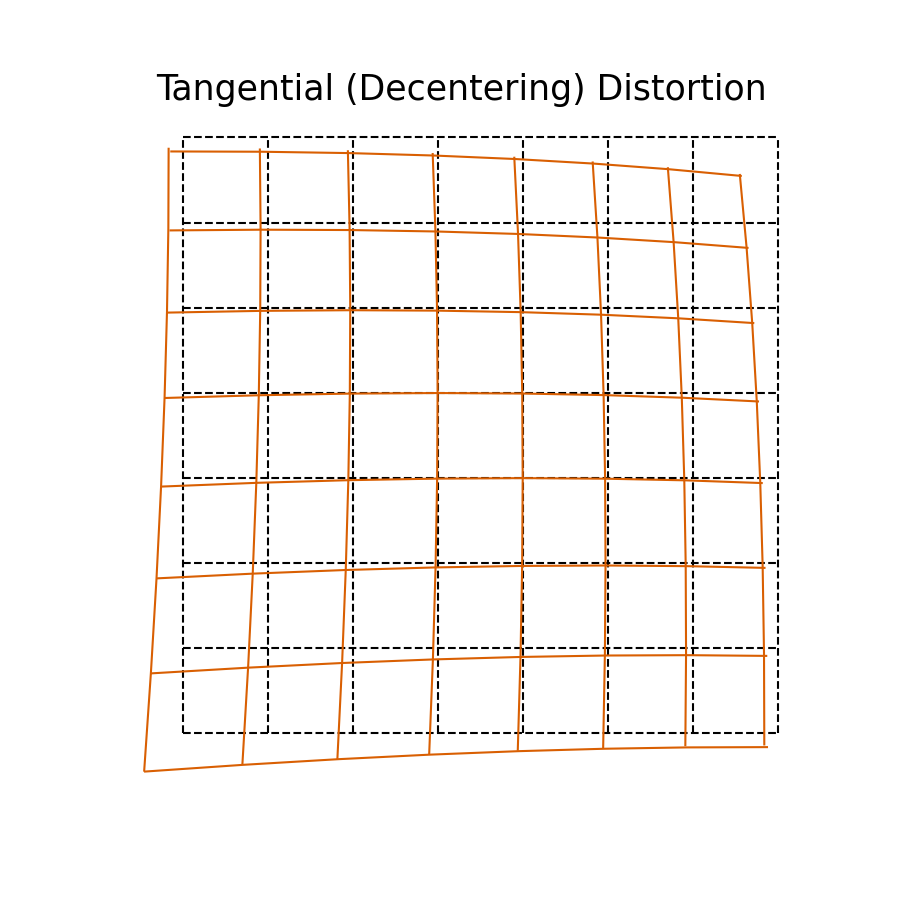
\includegraphics[width=4cm]{tang.png} }}%
    \label{fig:example}% 
    \caption{Impacts of Distortion on the Image Plane}
\end{figure}
\\ 

\subsection{Accounting for distortion}

The transformation process between raw and distorted pixels can be modelled using the 
formulas below: 

\begin{theorem}
    [Radial Distortion Equations] 
    \begin{align}
    x_{distorted} = x( 1 + k_1 r^2 + k_2 r^4 + k_3 r^6) 
    \\ y_{distorted} = y( 1 + k_1 r^2 + k_2 r^4 + k_3 r^6)    
    \end{align}
    
\end{theorem}


\begin{theorem}
    [Tangential Distortion Equations] 
    \begin{align}
        x_{distorted} = x + [ 2p_1xy + p_2(r^2+2x^2)]  
       \\ y_{distorted} = y + [ p_1(r^2+ 2y^2)+ 2p_2xy]
    \end{align}
    
\end{theorem}

As seen in the formulas the distortion is maginified through the following distortion coefficients: 
\begin{displaymath}
    Distortion \; coefficients=(k_1 \hspace{10pt} k_2 \hspace{10pt} p_1 \hspace{10pt} p_2 \hspace{10pt} k_3)
\end{displaymath}

By finding these components and transforming the pixels accordingly, the cameras are then 
completely calibrated. They are found by analyzing multiple images of known geometry and 
comparing the pixels in the camera with the real-world coordinates of the image. However, 
instead of completeing this process manually OpenCV, the framework being used, automates this 
process through built in functions, meaning only a conceptual understanding of lense distortion 
is needed to proceed. 

\section{Pixel Correspondence}

As mentioned prior, the pixel correspondence problem is the most studied are in the 
field of stereo vision and by extension, the main focus of this paper. The correspondence 
problem boils down to interating through each pixel in the left camera and finding the 
corresponding pixel in the right camera in a efficient and accurate manner. In this paper, 
two methods will be analyzed, a standard window based approach as well as a newer apprach 
using a optimization technique known as Dynamic Programming (DP). After implementation, the 
two appraches will both be tested using the same stereo system in order to reveal differences 
in accuracy and speed in order to determine the value in the usage of optimization algorithms, 
such as DP in computer vision. 

\subsection{Window Based SSD Disparity Estimation}

\subsection{Adaptible Window Optimizations}
\begin{remark}
  % paragraph paragraph name (end)
  Notes{\begin{enumerate}
        \item Now that the two cameras have been calibrated such that they are on a identical image plane wiht one another you can now find the disparity between pixels of the two images in order to find depth using the triangulation model.
        \item One way this may be done is through a window based method, where we search for the object selected in one image the seocnd by creating a window and linearly searching for identical pixels on the second image. This method may be done efficiently due to camera calibration as the pixel range is on the same scan line.
        \item We can explore other methods of stereo rectification if we have time as the computation is pretty simple. You would have the use
              a minimmum squared difference algorithm on the average intensity of the window.
      \end{enumerate}} % (fold)
  \label{par:Notes}


  % paragraph paragraph name (end)
\end{remark}

\subsection{Dynamic Programming Based Disparity Estimation}

\section{Implementation}

\subsection{Hardware}
\subsection{Program}

\section{Testing}

\section{Conclusion}

\section{Works Cited}

\section{Appendix}

\end{document}
